\documentclass{article}
\usepackage{graphicx}
\usepackage{amsmath}
\usepackage{amssymb}
\usepackage{subfigure}
\usepackage{epstopdf}
\usepackage{setspace}
\usepackage{authblk}
\usepackage[a4paper,left=1in,right=1in,top=1in,bottom=1.5in,footskip=.25in]{geometry}
\onehalfspacing

\newcommand{\nm}{\ensuremath{\,\textrm{nm}}}
\newcommand{\eV}{\ensuremath{\,\textrm{eV}}}
\newcommand{\uM}{\ensuremath{\,\mu\textrm{M}}}
\newcommand{\uW}{\ensuremath{\,\mu\textrm{W}}}
\newcommand{\meV}{\ensuremath{\,\textrm{meV}}}

\title{In situ tuning of nanorods' plasmon through oxidative etching with KCN}
\author[1]{Aquiles Carattino}
\author[2]{Saumyakanti Khatua}
\author[1]{Michel Orrit}
\affil[1]{Leiden Institute of Physics, Leiden, The Netherlands}
\affil[2]{Indian Institute of Technology- Gandhinagar, Ahmedabad,  India}
%\ead{Corresponding Author Email Address}
%\cortext[a]{khatuask@iitgn.ac.in, Orrit@physics.leidenuniv.nl }
\begin{document}

\maketitle
\abstract{This is the abstract}

\section{Introduction}

Gold nanoparticles exhibit enhanced absorption and scattering cross sections
ranging from the visible to the near infra red. This property is closely related
to the surface plasmon (i.e. a collective oscillation of conduction electrons)
that in turn depends on the shape of the particles. For the case of gold
nanorods (AuNR) their surface plasmon resonance (SPR) energy depends on the
aspect ratio (AR) of the particle and can be found between $550\nm$ for
spheres (AR of $1$) to even above $800\nm$ for very elongated
particles.

The surface plasmon presents great opportunities in (bio-)
sensing\cite{Zijlstra2012}, enhanced spectroscopies\cite{Sivapalan2013},
photothermal therapy\cite{Zhao2014}, and concentrating light below the
diffraction limit\cite{Zijlstra2011}. Success in many of these applications
requires precise and in situ control over the nanoparticles' plasmon resonance
energy. For example, maximum fluorescence\cite{Khatua2014} or Raman
enhancement\cite{McFarland2005} is achieved when the nanoparticle's plasmon
resonance is tuned to excitation laser wavelength or efficient photothermal
therapy requires nanoparticles' SPR to be tuned to NIR to minimize the damage to
healthy cells\cite{Alkilany2012}.

Typically, SPR is tuned by carefully manipulating the shapes of nanoparticles
during their synthesis. Particularly useful are the rod-shaped particles, whose
resonance can be tuned from $600\nm$ to over $1000\nm$ by changing their aspect
ratios through carefully adjusting the concentrations of gold-seed and silver
nitrate during the seed-mediated growth synthesis method\cite{Vigderman2012}.
Many other nanoparticles shapes, such as nanoprisms, nanorice, nanocubes,
nanoshells, etc. have been synthesized with their plasmon resonances covering
entirely the spectral range from visible to near-IR\cite{West2003}. Wet-chemical
synthesis methods, however, generally yield a broad distribution in
nanoparticles sizes and/or shapes, which hinders precise and reproducible tuning
of nanoparticles SPR. Furthermore these methods do not provide any in-situ
adjustment of SPR; any change of which would require a new synthesis.

Recently, new methods have been developed to tune nanoparticles' SPR after their
synthesis. These approaches can be divided into two broad categories: ($1$) The
first group of methods tune the refractive index of the medium using an electric
or magnetic field\cite{Kossyrev2005}. The advantage of these methods is that the
SPR shift is reproducible and reversible. However the tuning range is rather
limited and the continuous tuning within this range is difficult to achieve.
($2$) The other set of approaches rely on controllably inducing shape
modifications of the nanoparticles to tune the plasmon resonance through
chemical or physical means. For example, thermal reshaping was induced by
illuminating the nanoparticles with an intense, pulsed
\cite{Link2000}\cite{Horiguchi2008} or continuous laser\cite{Yorulmaz2012}.
Increasing the particles' temperature therefore leads to change in shape,
favoring those conformations with a lower surface energy (i.e.
spheres over rods, etc.). Chemical reshaping is also possible and was the focus
of several studies\cite{Carbo-Argibay2007}
\cite{Rodriguez-Fernandez2005} \cite{Jana2002}. In those cases, the capping
agent will induce different reactivities on the sides than on the tips of the
particles; because of a higher curvature\cite{Yuan2015} the the tips are
normally more susceptible to chemical reactions, leading to an anisotropic reshaping
shortening the long axis or softening any high-curvature region. In both cases
(laser or chemical induced reshaping) the outcome is a blue-shift of the surface
resonance peak.

% The chemical reshaping is normally performed in bulk, with the nanoparticles
% dispersed in solution. Another group has studied how the chemical reactivity of
% gold \cite{Ni2012} can be altered by exploiting the plasmon resonance. This is
% achieved mainly through changes in the surrounding temperature; it has to be
% noted that in these experiments the surfactant was present as for the bulk
% experiments. In another work\cite{Tsung2006}, high resolution TEM images allowed
% to show that the crystal structure of individual particles is preserved after
% oxidation inducing a shortening of the long axis of over $10\nm$. A common trend
% in the vast majority of these works is that nanorods tend to reshape into
% spheres, giving rise to a blue shift of the longitudinal plasmon resonance.

Here we present a new approach for precise and in-situ tuning of plasmon
resonances of single gold nanorods isolated and immobilized over a glass
surface. A nanorod's plasmon resonance is tuned over $130\nm$ (starting from
$650\nm$ up to $780\nm$). Our method exploits well known chemistry between gold
and potassium cyanide (KCN), to controllably etch gold atoms from the
nanoparticle and thereby change its aspect ratio. We note that unlike many of
the previous studies, here we observe a red-shift of SPR on gold nanorods.
Our simulations based on the discrete dipole approximation method attributes
this red-shift to symmetric etching of gold nanorods from all sides resulting in
overall increase of aspect ratio. This is in contrary to previous studies, where
the etching was preferred at the tips, resulting in an overall decrease of
aspect ratios. The symmetric etching of gold nanorods is also verified from
scanning electron microscopy (SEM) images.

% Our experiments are new in performing both single-particle studies while
% removing the surfactant from the equation. Controlling the concentration of KCN
% allows to fine tune the plasmon peak position of individual particles, without
% hindering the known optical properties of them. Moreover we show that only a few
% thousand molecules of KCN have to react with the nanoparticle in order to cause
% an observable change in the plasmon position.

\section{Experimental method}
\begin{figure}[p]
 \centering 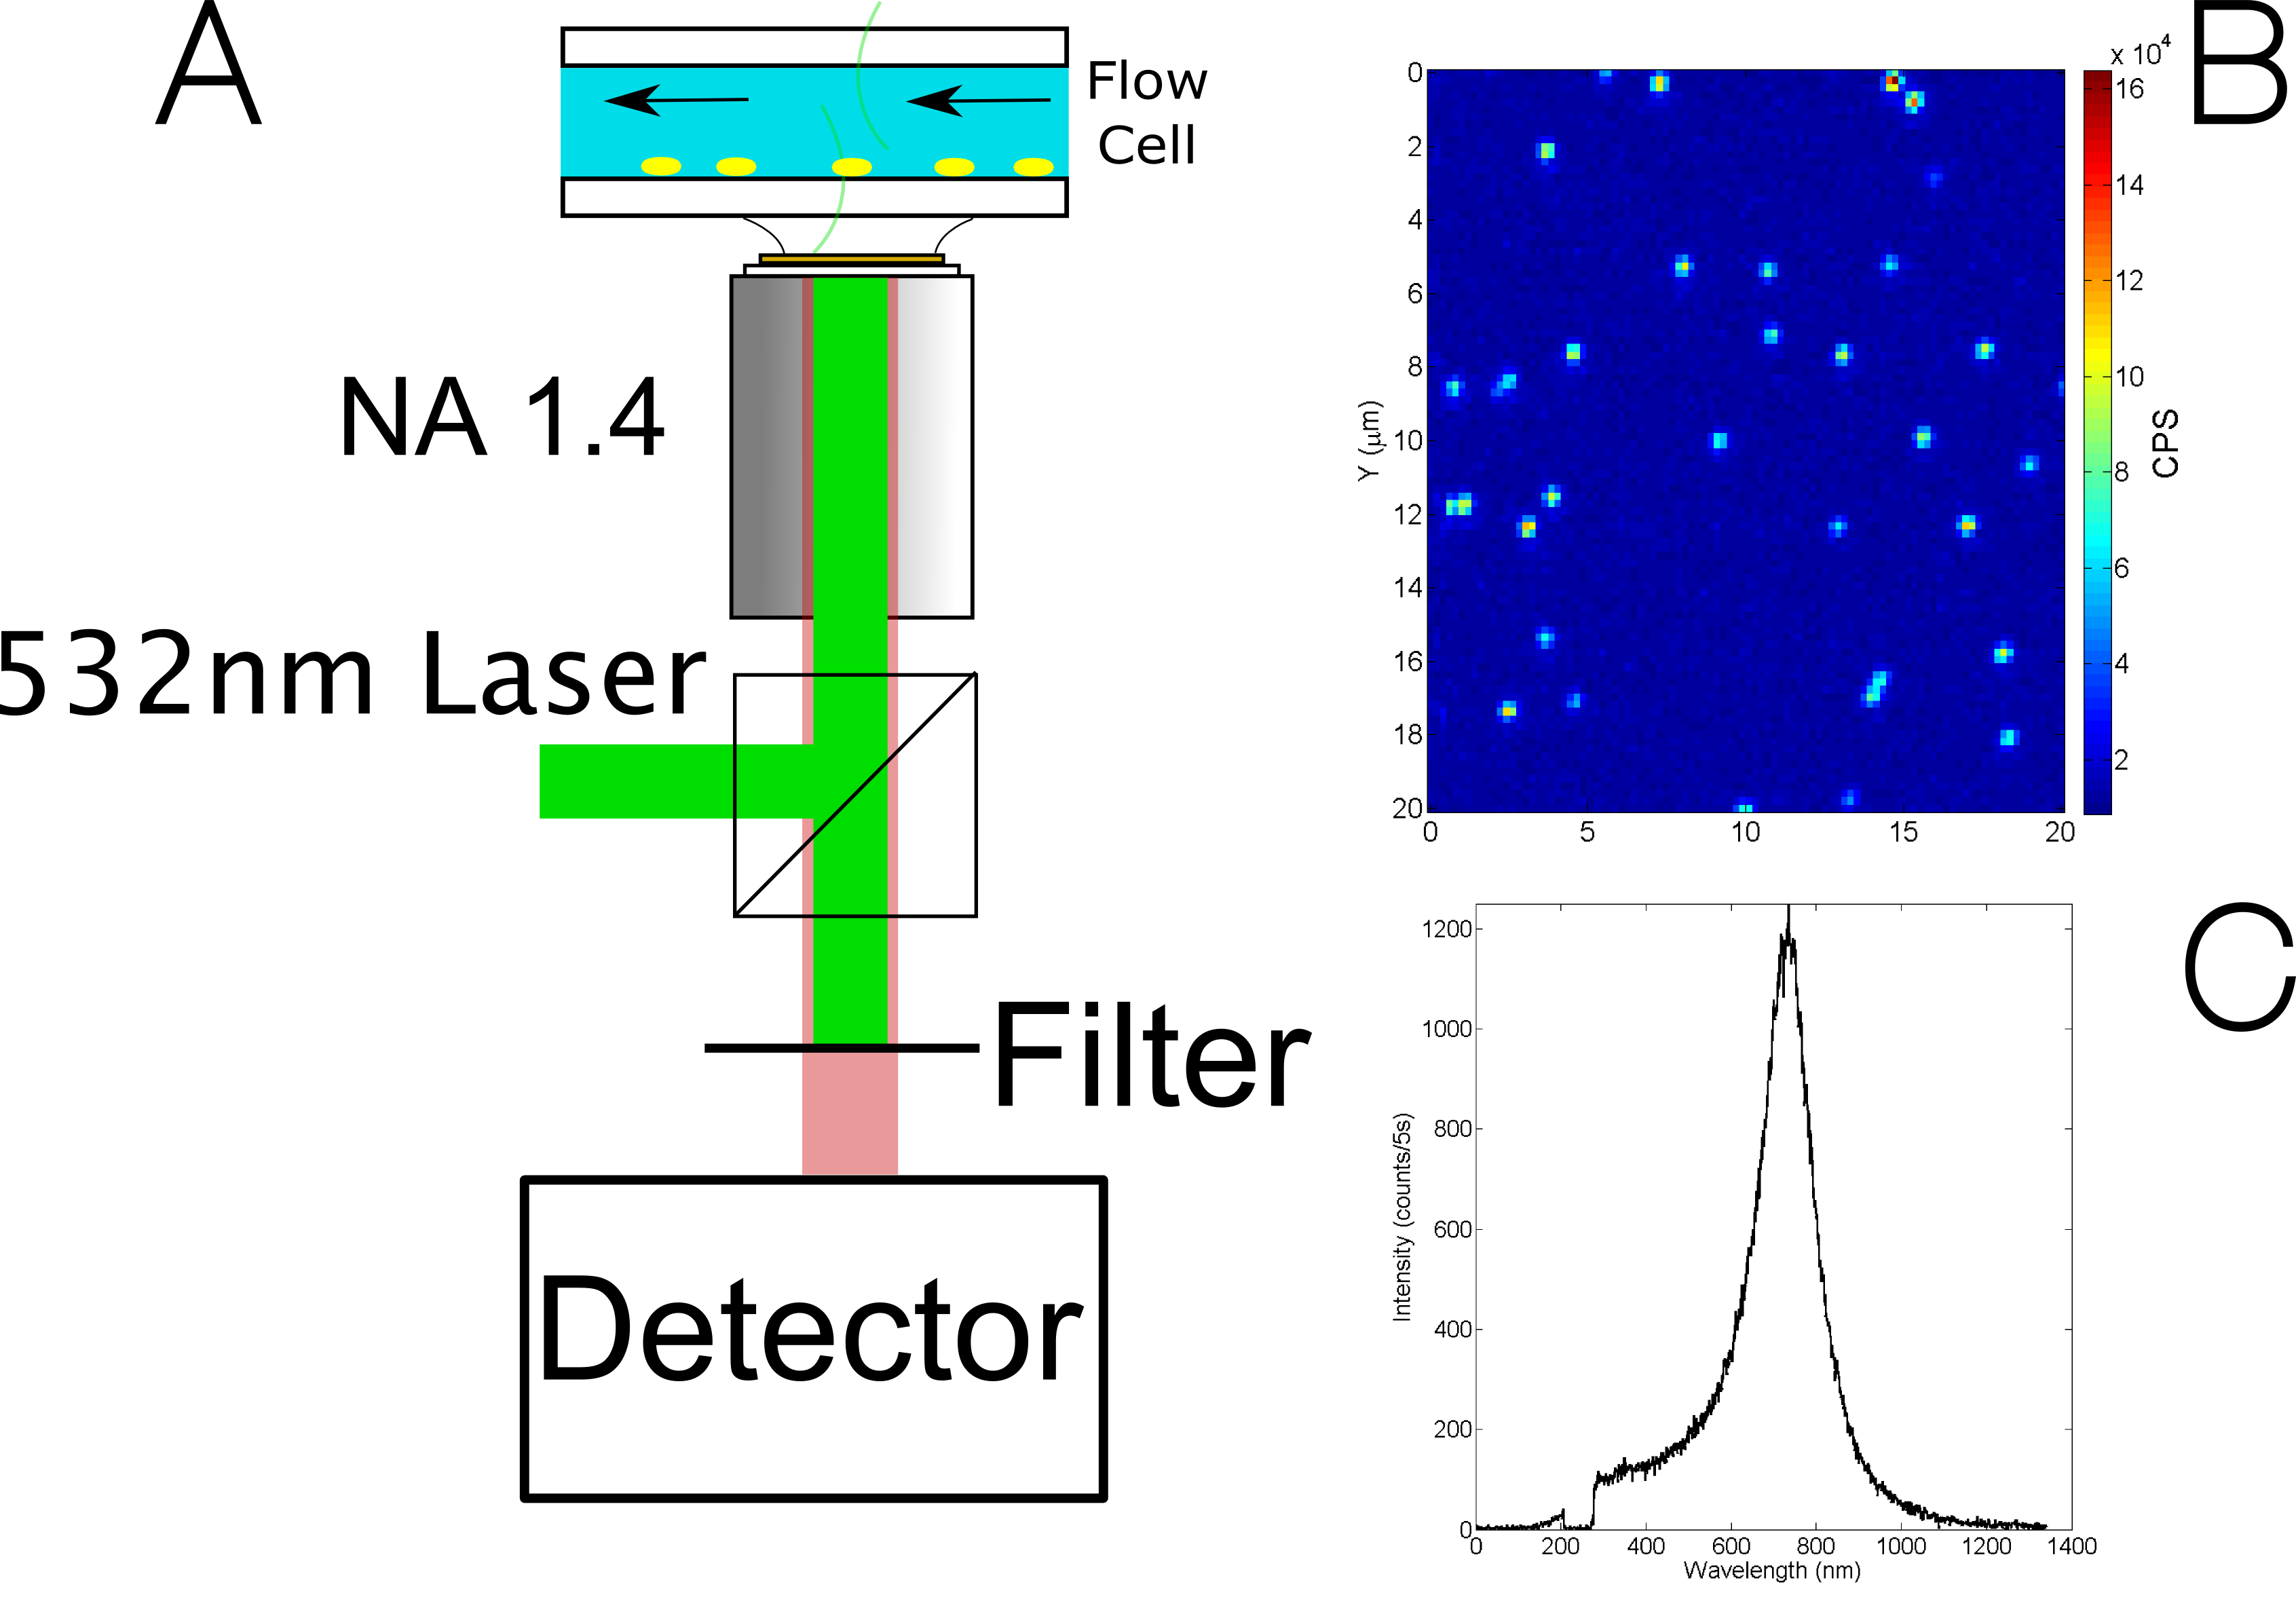
\includegraphics[width=0.45\linewidth]{Figures/01_Setup/setup_1.png}
 \caption{Experimental setup and examples of the observations. A) Simplified
 schematic of the confocal microscope employed during the measurements. B) A
 typical 1-photon luminescence raster scan of the sample immersed in
 water, before etching and C) luminescence spectrum of a single rod.}
 \label{fig:setup}
\end{figure}

Gold nanorods were synthesized by following standard seed-growth method\cite{Nikoobakht2003}.
The average size of the nanorods was $60\nm\times 25\nm$ and their SPR is
located at $650\nm$ in water (SI figs: SEM image and bulk extinction of
nanorods as synthesized).

Single-particle measurements were done on a home-built confocal microscope
(Figure \ref{fig:setup}). A $532\nm$ laser was used for exciting the particles.
The excitation power was $300\uW$ at the back focal plane of the objective
(Olympus $60\times$, $\textrm{NA}\,0.9$ air). The luminescence signal was then
filtered with two $532\nm$ notch filters and was detected by either an avalanche
photodiode or a liquid nitrogen-cooled CCD-spectrometer (Acton $500\textrm{i}$).
The images were acquired by scanning the sample across a tightly focused laser
beam using a XYZ piezo scanning stage (PI Nano Cube).

The samples were prepared by spin casting a suspension of AuNR on clean
coverslips and thoroughly rinsing them  with Milli-Q water and placed in an
ozone cleaner for eliminating the excess of CTAB. Afterwards the samples are
placed in a flow-cell; the initial spectra is taken with the rods immersed in
Milli-Q water (see for example Figure \ref{fig:setup}.c). This initial
characterization allows us to discard clusters of rods\cite{Funston2009}. Next,
a solution of KCN was flowed into the cell with concentrations ranging from $3\uM$ to $80\uM$. In each
case the spectra of approximately $10$ different particles are acquired
consecutively after focusing on each one. The time resolution varies according
to the exposure time and number of particles; in this work a spectra of each
particle is taken at least every minute.

\section{Results}

Figure \ref{fig:setup}.b shows a typical one-photon-excited luminescence image
of gold nanorods isolated on glass surface and covered with water.
Approximately, $90\%$ of the diffraction-limited bright spots originate from
single gold nanorods. This was confirmed by acquiring their luminescence
spectra, which show narrow Lorentzian lineshapes\cite{Funston2009}. Figure
\ref{fig:setup}.c depicts a typical one-photon excited luminescence spectrum of
a single gold nanorod.

\begin{figure}[p]
 \centering 
 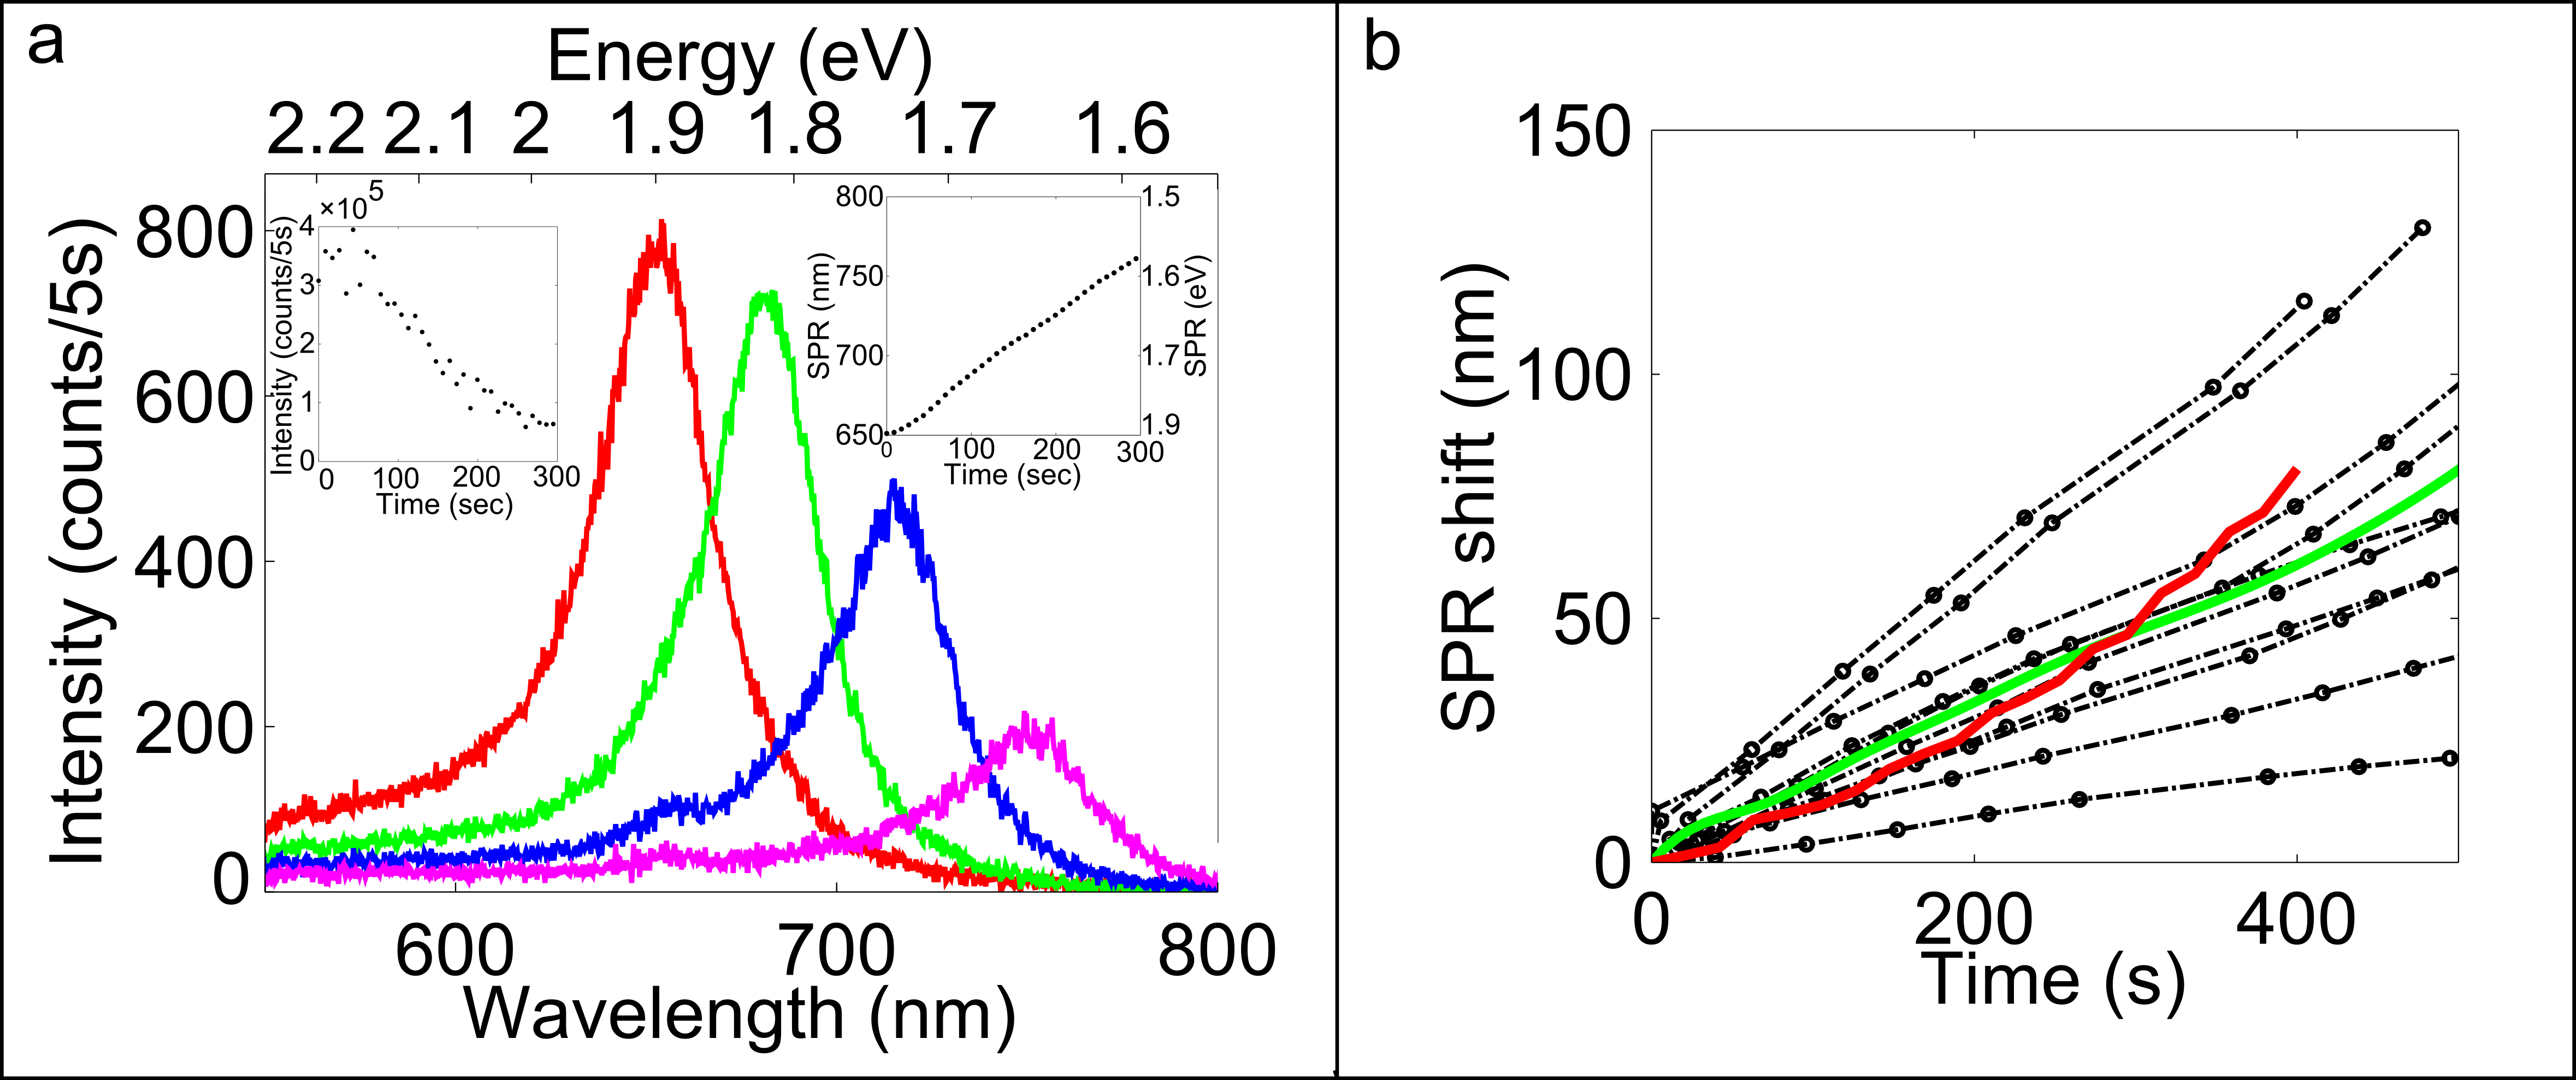
\includegraphics[width=0.95\linewidth]{Figures/02_Experimental/Experimental.png}
 \caption{Single-photon luminescence spectra of gold nanorods immersed in $20\mu
 M$ KCN. A) Plasmon shift of a single rod. The curves are displayed at $70s$
 intervals. The insets display the intensity of the peak as a function of time
 and the resonance wavelength respectively. B) Shows the peak shift time-trace
 for 9 different particles. The red curve is the average while the green is
 the best fit from discrete dipole simulations with etching rate fixed at
 $1\nm/min$}
 \label{fig:plasmon_single_rod}
\end{figure}

Figure \ref{fig:plasmon_single_rod}.a shows the one-photon luminescence spectra
of a gold nanorod immersed in $20\uM$ KCN at intervals of $70\,\text{s}$. We
clearly observe a gradual red-shift of the nanorod�s plasmon resonance by
$100\nm$ over a time interval of $300\,\text{s}$. This red-shift is also
associated with a decrease of photoluminescence intensity by factor of $4$. A
more detailed analysis shows that the nanorod�s plasmon resonance wavelength
(calculated from fitting with a lorentzian function) varies almost linearly with
respect to time (inset of Figure \ref{fig:plasmon_single_rod}.a) We note the
presence of an additional shoulder peak at $650\nm$ ($1.9\,\eV$) which is more
prominent for the less intense curves and is due to Raman scattering of
water\cite{Snow1985} that could not be completely removed when subtracting the
background (see SI for the spectra of the background). 

We find the same trend for all the nanorods that were studied. Our results are
summarized in \ref{fig:plasmon_single_rod}.b, which shows the shift of plasmon
resonance wavelengths as a function of time for nine different rods (the dashed
lines). Each nanorod shows a red-shift of the plasmon resonance wavelength,
which varies almost linearly with time irrespective of their initial resonance
energy. The rate of SPR shift, however, varies significantly from particle to
particle with the fastest one being $15\nm/\textrm{minute}$ to the slowest one
of $2\nm/\textrm{minute}$. The green curve in Figure
\ref{fig:plasmon_single_rod}.b is the average of all the shifts; since the
spectra of each particle were acquired sequentially, we interpolated the values
of the shift at given times with a cubic spline.

The chemistry between gold and potassium cyanide is well known and is being used
for gold mining, electroplating, organic synthesis, etc. Gold reacts with
aqueous KCN in presence oxygen to form $\textrm{Au(CN)}_2^-$, which is soluble
in water. The reaction can be written as follows
\begin{equation*}
4\textrm{Au} + 8\textrm{KCN}^-+\textrm{O}_2 + 2\textrm{H}_2\textrm{O}
\leftrightarrows 4K\textrm{Au(CN)}_2^-+4\textrm{KOH}^-
\end{equation*}
In our experiment formation of $\textrm{Au(CN)}_2^-$ will result in etching of the gold
atoms from the nanorods, as has been reported previously\cite{Jana2002}.  

The etching of gold atoms from a nanorod has two effects: Firstly, the nanorod�s
volume will decrease gradually with longer reaction time. This is consistent
with our observation that the one-photon-luminescence intensity decreases with
time. Secondly, the aspect ratio of a nanorod can either decrease or increase
depending on the preferred direction of etching. Nanorods� aspect ratio will
decrease with time when the reaction happens preferably from the tips. This is
indeed the case for nanorods protected with CTAB and dispersed in
solution\cite{Jana2002}. CTAB binds weakly to the tips compared to the sides and
therefore leaves the tips more susceptible for chemical
reactions\cite{Caswell2003}. The consequent decrease of aspect ratio yields a
blue shift of plasmon resonance\cite{Link1999}. In a second case, etching happens
isotropically from all sides and tips resulting in an overall increase of the
nanorod's aspect ratio. This is the more likely scenario in our experiment as
the nanorods� surface does not have any protective CTAB bi-layer.

Numerical simulations based on the discrete dipole approximation model were
performed to further confirm that the red shift of plasmon resonance is indeed
due to isotropic etching of the nanorods. The initial dimensions of the
particles were fixed at $25\nm\times60\nm$ which coincided with the median
dimensions of the distribution of sizes of the nanoparticles (see SI). These
simulations are carried out in steps of $0.5\nm$ for a total of $10\nm$ (i.e.
the minimum particle size is $15\nm\times 50 \nm$). Figure
\ref{fig:simulations}.a shows the scattering spectra of the particle at
different etching intervals. We clearly observe a red-shift of the plasmon
resonance wavelength, as was observed in our experiment. The insets of the
figure show the decrease of the integrated scattering spectrum as a function of
the etching and the detailed time-evolution of the SPR obtained from the fitting
of the peaks with a lorentzian function. Both are compatible with the
experimental observations. Furthermore it is possible to fix the etching rate to
best approximate the average plasmon shift. These results are displayed as the
red curve in Figure \ref{fig:plasmon_single_rod}.b. The best approximation to
the average is found when the etching rate is set to $1\nm/\textrm{min}$.

\begin{figure}[p]
 \centering
 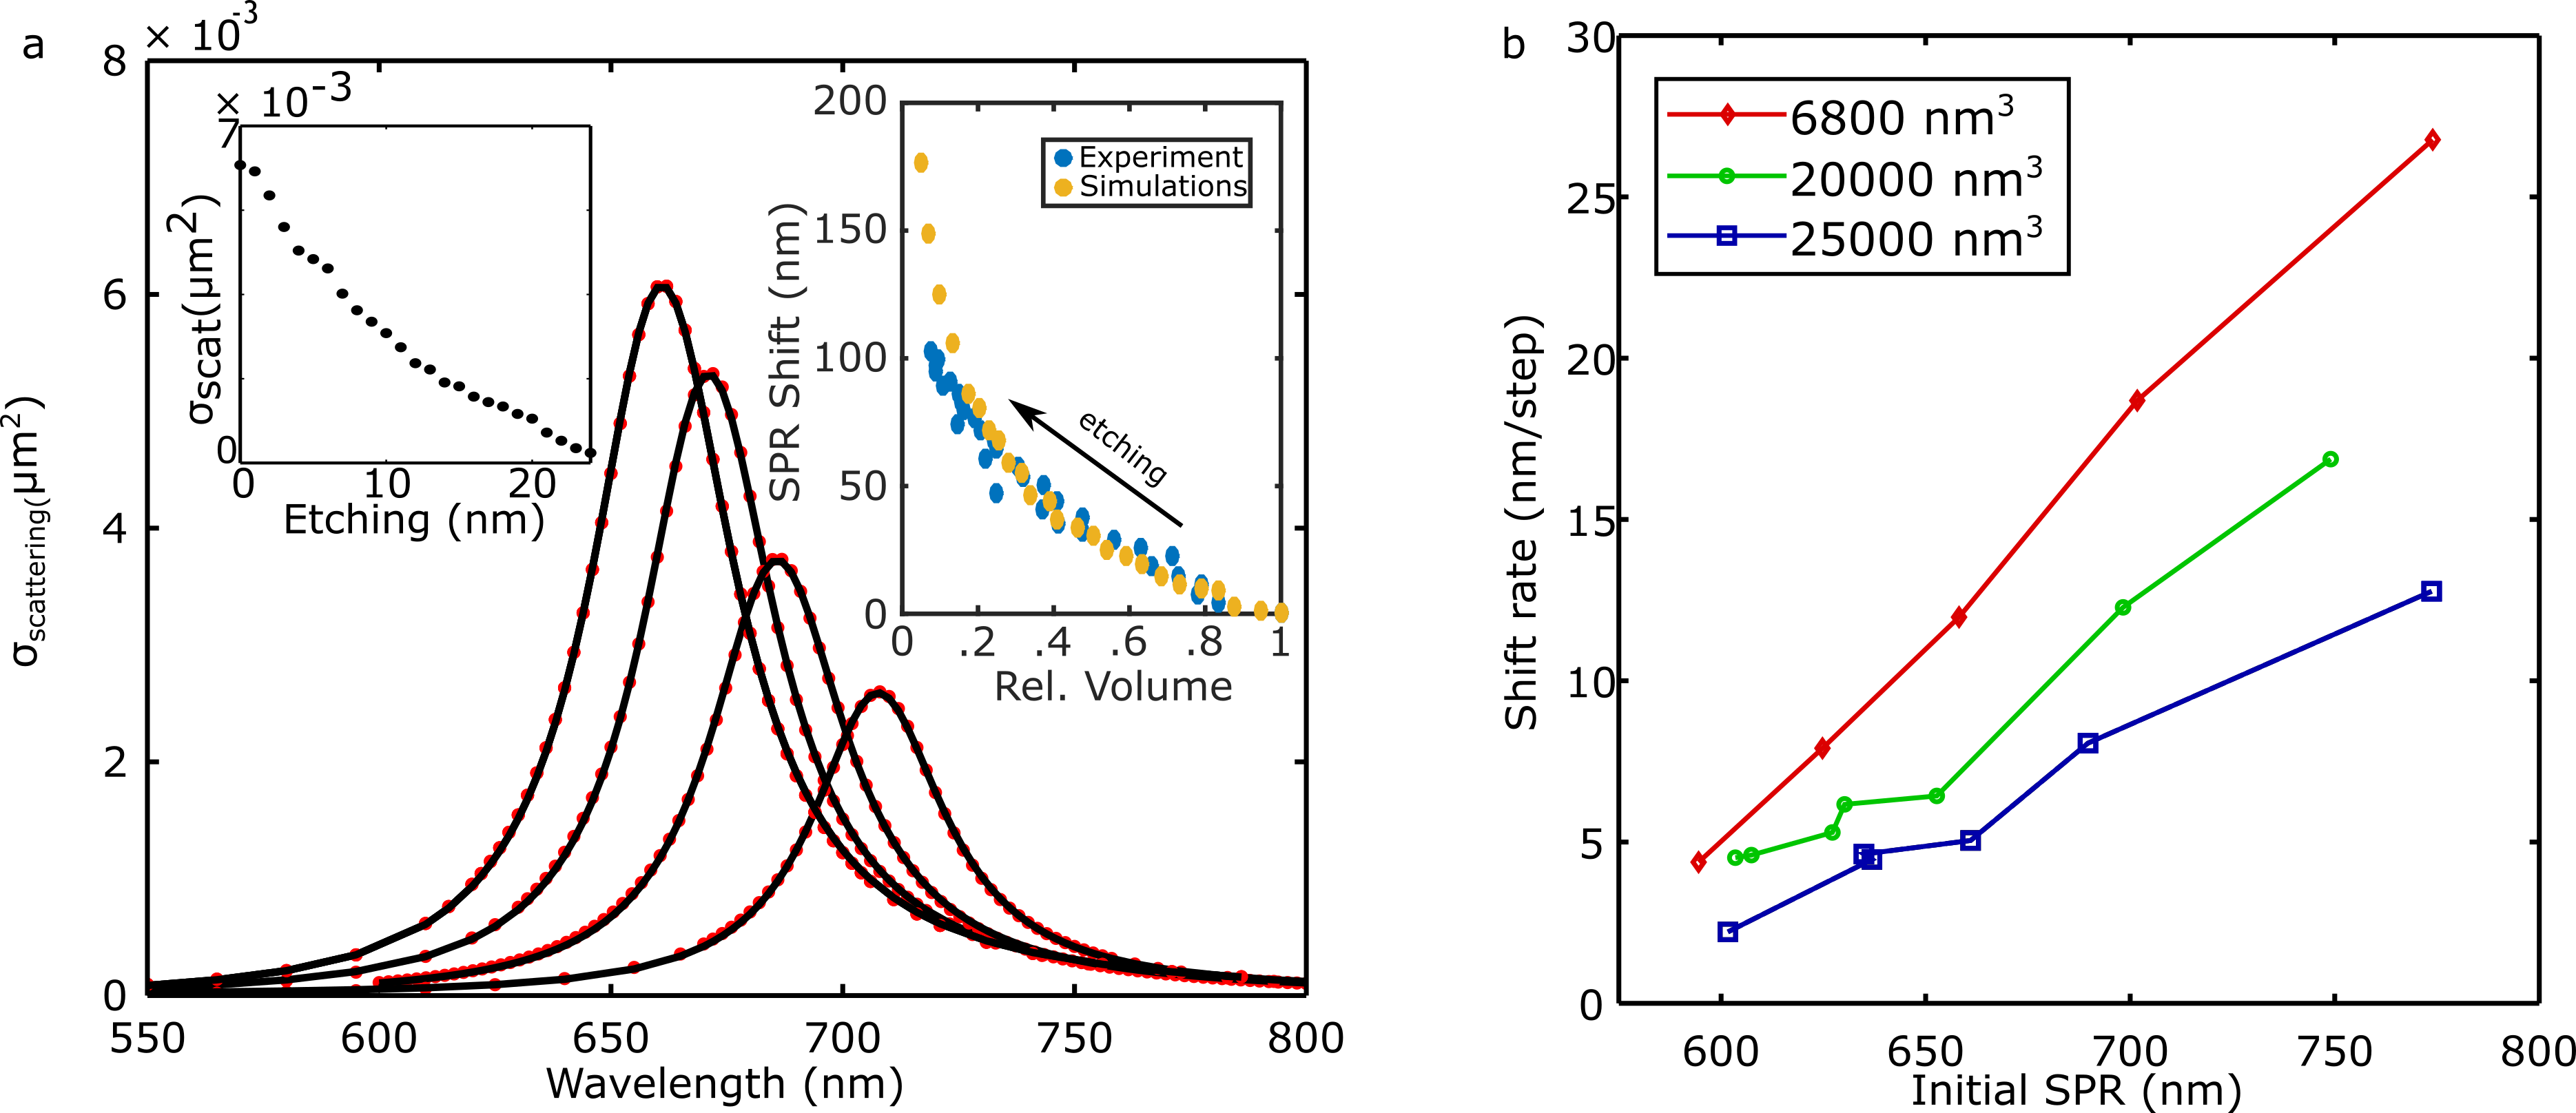
\includegraphics[width=0.95\linewidth]{Figures/02_Simulations/simulations.png}
 \caption{Simulated plasmon spectra at different etching steps. A) Examples of
 the curves obtained at different simulations steps. The black curves are
 fittings with lorentzians. The insets show the intensity and the SPR as a
 function of simulation step. B) Shows the shift rate as a function of the
 initial volume of the particle. C) Shift rate for particles with fixed width
 ($25\nm$) and variable length as a function of their initial SPR. }
 \label{fig:simulations}
\end{figure}

Furthermore the simulations allow to study the different shift rates that were
present in the experimental results. Figure \label{fig:simulations}.b shows the
different shift rates as functions of the initial volume of the particles. The
shift rate is defined through a linear fit of the plasmon shift as a function of
etching steps. There is a great variability of results even for particles with
similar volumes. Figure \label{fig:simulations}.c shows the shift rate as a
function of initial SPR for particles with a fixed width ($25\nm$) and
different lengths. It can be seen that particles with higher aspect ratios
(higher SPR wavelengths) tend to shift more rapidly. This is also observed in
the inset of \label{fig:simulations}.A, where the shift as a function of
simulation step is clearly increasing more rapidly conform the etching
progresses. The simulations therefore prove that both the initial volume and SPR
will have a role in the rate at which the plasmon peak shifts. 


\begin{figure}[p]
 \centering
 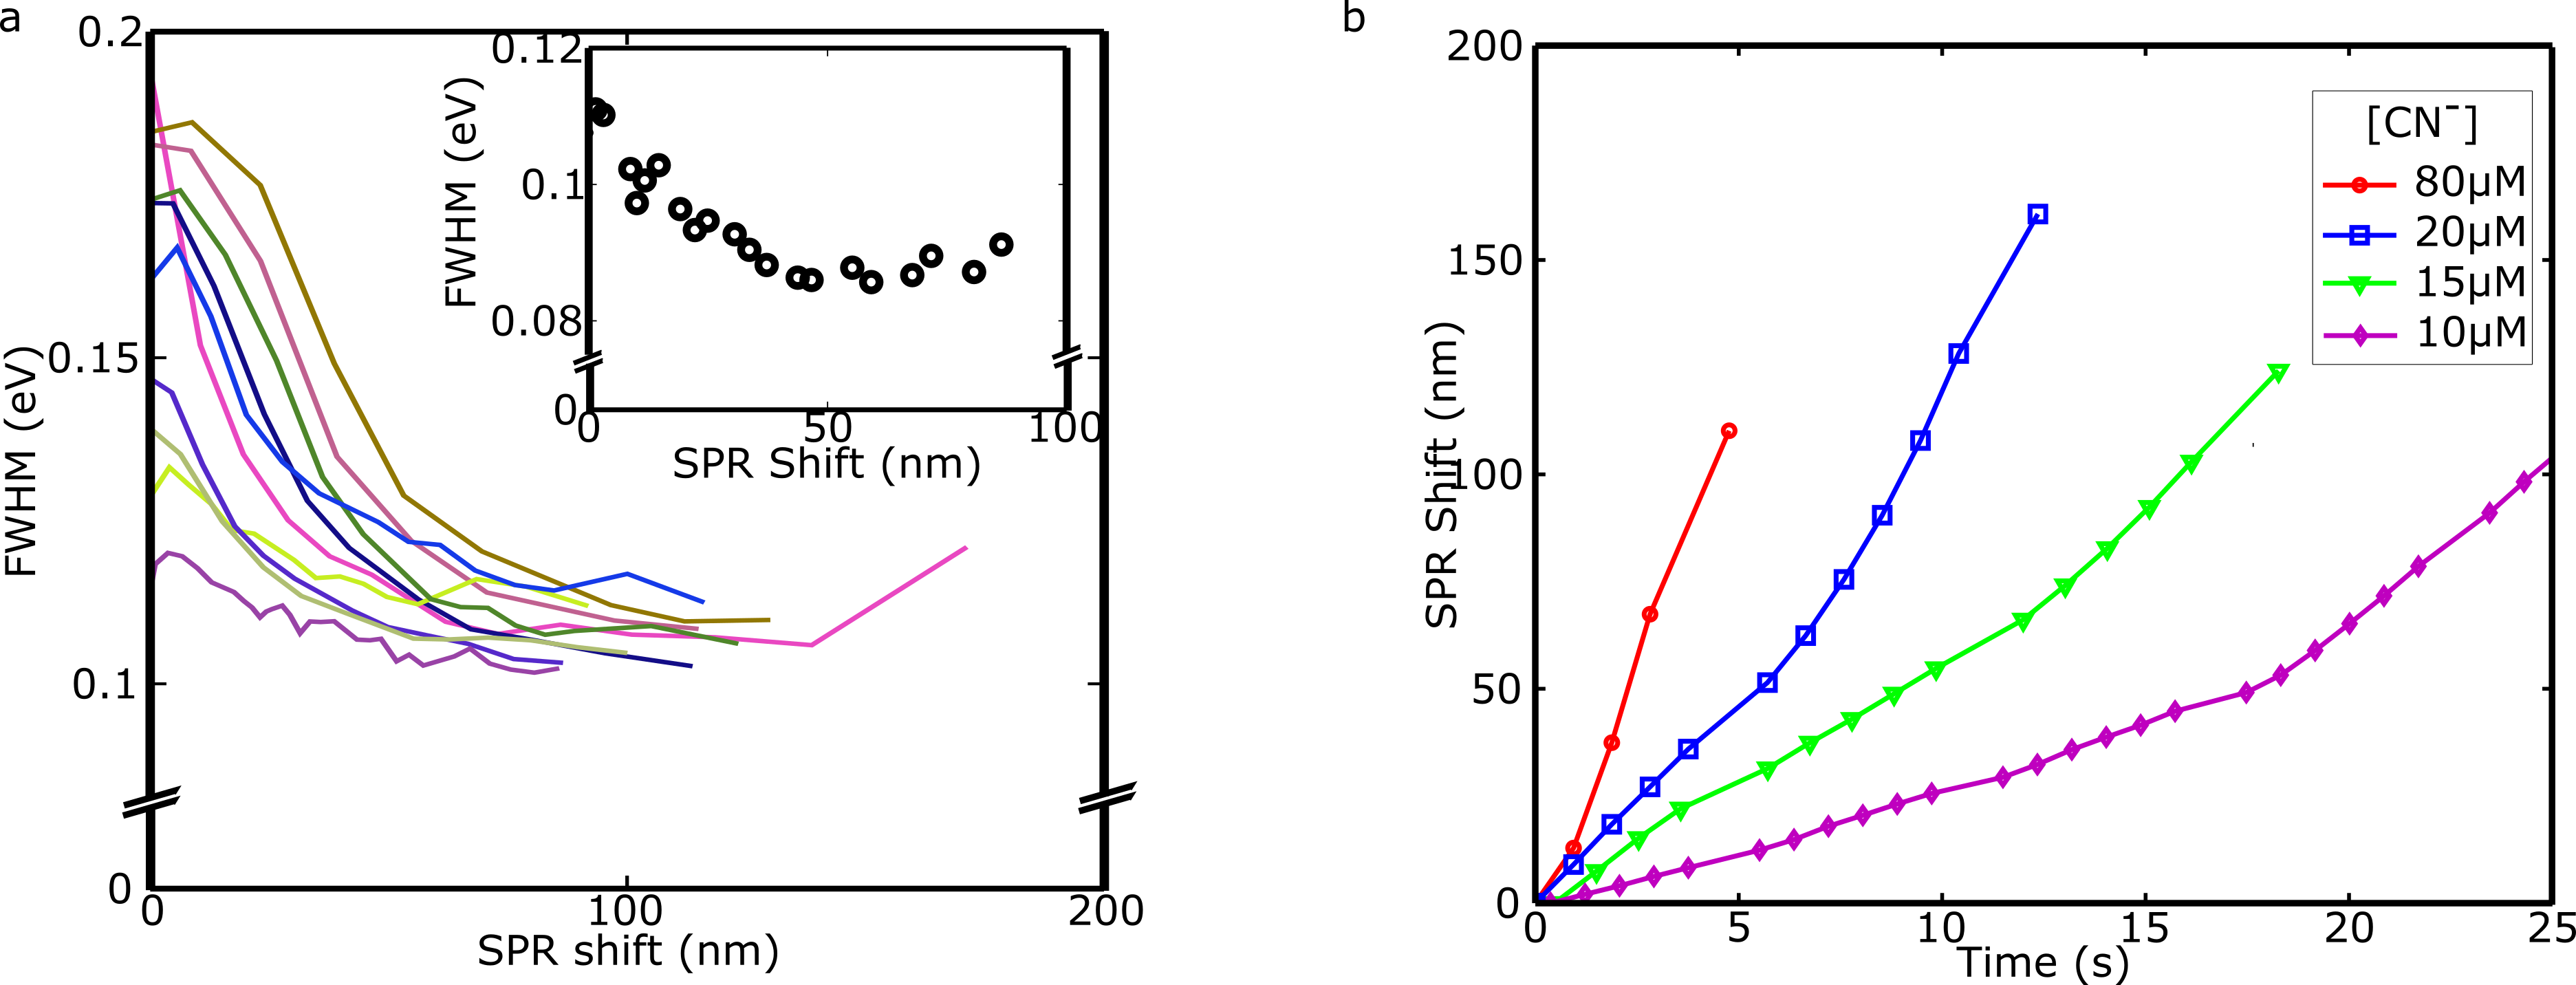
\includegraphics[width=0.95\linewidth]{Figures/03_Shifts/shifts.png}
 \caption{A) Plasmon FWHM of eight different particles immersed in $20\,\mu M$
 KCN as a function of their plasmon shift. The inset shows the results from the
 simulations carried out with the ADDA package. B) SPR Shift as a function of
 time for particles with the same initial SPR at different KCN concentrations.
 The inset shows the shift rate of these same particles.}
 \label{fig:FWHM}
\end{figure}

Figure \ref{fig:FWHM}.a shows how the FWHM of the plasmon peak decreases while
the shift increases for several nanorods immersed in $20\uM$ KCN. Note the units
of the plot, since it is not trivial the use of wavelengths for the FWHM, we
show these results in energy scale. At the beginning of the reaction there is a
rapid diminishing of the width, probably due to the elimination of defects from
the surface of the particles. Then a minimum is reached for shifts between
$75\nm$ and $100\nm$.  While the reaction continues, the width starts to
increase; this means that the reshaping at some point will start having an
effect on the shape of the particle and because of the reduction in particle
volume, other dephasing effects may start being relevant (for instance, surface
scattering). This is often encountered for shifts above $100\nm$, but depends on
the particle initial size and shape. The inset of the Figure shows the FWHM
obtained from the simulations for a $25\nm\times60\nm$ nanorod. The width
decreases with the shift slightly slower than in the experiment but the trend is
similar to the observed. 

The observed and simulated decrease of width can be explained considering that
both the radiative and non-radiative damping decrease during the etching
process. The radiation damping scales as the volume of the
particle\cite{Wokaun1982} and therefore will decrease while the cyanide etches
gold atoms from the particle. On the other hand, we observe that the energy
distance between the longitudinal plasmon peak and interband transitions in gold
increase during the etching process. Therefore the non-radiative damping
mechanisms in the particle become less efficient\cite{Sonnichsen2002}. Both
effects combined explain the fast diminishing in plasmon width that is observed.

Figure \ref{fig:FWHM}.b shows the plasmon peak shift as a function of time
for various KCN concentrations for particles with a plasmon peak position of
roughly $630\nm$. As shown for the simulations (Figure
\ref{fig:simulations}.c), the initial SPR will have a role on the etching rate,
therefore it is important to choose particles that are similar to each other.
The volume of the particles can be approximated by the intensity of the
luminescence, however is more prone to errors (different excitation intensities,
not perfectly focused on the particle, etc.) The timetraces of the peak position
clearly show that the shift rate is proportional to the concentration of KCN.
This result is also shown in the inset, where the shift rate is defined as
previously and plotted as a function of the concentration of KCN.

From these results and adapting the etching model we estimate that the reaction
rate can be as low as $700$ atoms per second for a KCN concentration of $10\uM$.
In the experiments performed at $3\uM$ concentration, the particles chosen
didn't have a plasmon close to $630\nm$ and therefore are not shown; if in any
case the extrapolation still holds true for this low concentrations it would
yield a rate of just $200$ atoms per second. Inverting the relationship, the
plasmon peak shift while gold reacts with KCN happens at a rate of roughly
$0.5\cdot 10^{-6}\,\textrm{eV}/\textrm{atom}$.

% Every particle can be slightly different from another, not only because of its
% aspect ratio (and plasmon peak position) but also because of the presence of
% surface impurities. This was shown already in Figure \ref{fig:FWHM} where the
% FWHM decreases steeply at the beginning. The distribution of particle sizes and
% aspect ratios will in turn lead to different shift rates that will cause a
% broadening of the peak distribution after etching. These results are for
% particles immobilized on the coverslip and with all the surface capping washed
% out, leading to an isotropic etching. In bulk, where the rods are freely
% difussing and the surfactant is still present, the results are different.

Samples of the same nanorods are prepared for SEM imaging by drop casting the
same solution of rods. The images were acquired before the etching, after
$2\,\textrm{min}$ submersed in KCN and after $4\,\textrm{min}$. When particles
are isolated from each other, the model of the isotropic etching seems
appropriate, as the shape is preserved. It has to be noted, however, that for
aggregates of particles this no longer holds, and rods start to lose their
shape (see Supporting Information for SEM images.) Calculating the distribution
of sizes of the particles shows a slight increase in the aspect ratio but this
is however obscured by the broad distribution of values (even before starting
the etching). Averaging around $300$ different particles at each interval yields
an etching constant of $0.5\nm/\textrm{minute}$, consistent with the optical
observations, not only of the plasmon shift but also of the diminishing
intensity as a function of time.

The presence of the surface is another aspect that may explain the difference
between the bulk and single-particle results. The surface would prevent the
reaction of gold with KCN from happening on one of the sides of the rods. By
definition this implies a non-isotropic model. On the other hand it would also
imply that the shape of the rods is not preserved since they would get
flattened. If this would be the case, the FWHM of the rods is expected to
increase but it was not observed, at least for the first couple hundreds
$\textrm{meV}$ of shift. The SEM images do not allow to assess this question
because there is no information on the third axis (perpendicular to the
surface). Experiments performed in an optical tweezer away from the surface as
done in Ref \cite{Ni2012} but without the capping agent would involve in
addition the use of microfluidics and therefore are much harder to perform.


\section{Conclusions}
In this work we have shown a simple method that allows the tuning of the plasmon
peak position of single gold nanorods with nanometer accuracy and over the range
of $100\nm$ ($300\meV$). More importantly, it is shown that
the rodlike shape is preserved for these shifts and therefore the well known
optical properties of the nanoparticles are not dampened. Moreover the absence
of the capping agent also works in favor of the proposed mechanisms in previous
works.

The experiments allow to record the plasmon peak with a relatively high temporal
and spectral accuracy, allowing us to stop the reaction when the resonance is at
the desired value. Both SEM images and the study of the FWHM of the longitudinal
resonance allow us to confirm that the shape of the rods is being preserved. The
agreement between the simulations assuming an isotropic etching and the
experimental results not only shows the link between both measurements but also
provide a way of predicting the behaviour of the plasmon peak for different
rods.

It is also found a great distribution of the rate at which the plasmon peak
shifts for different particles under the same experimental conditions. This can
be attributed to the initial aspect ratios of each particle. Sphere-like
particles will show a small shift due to the fact that the aspect ratio is
constant while under isotropic etching. The more elongated particles, on the
other hand, will have a much steeper increase in aspect ratio while being
etched. The majority of the rods present in the samples studied belong to an
intermediate position, with their resonance at $650\nm$ (aspect ratio
of $2.4$). The simulations agree with this statement, however experimental date
to further confirm this hypothesis is needed. 

The role of the capping agent has largely been studied and has always been held
responsible for the observations both in chemical etching\cite{Yuan2015} and for
photothermal reshaping\cite{Horiguchi2008}. Avoiding the presence of the
passivating layers is impossible in suspension, since gold nanoparticles would
aggregate. Our results do not only provide a method for changing the plasmon
resonance after the synthesis and in-situ, but also provide evidence that
supports previous observations regarding the effect of the curvature and the
accessibility of KCN to the surface of the particle. We also show that
single-particle experiments open new ways of controlling the particle shape.

A simple approximation of the reaction rates show that the dissolution of just a
few thousand atoms in the gold nanoparticle is enough for detecting a change in
the luminescence spectra. This method is not aimed at pushing the detection limits
of KCN (or other substances) via plasmonic structures, but still has proven to
be highly efficient. A better approach to sense plasmon shifts is to detect
changes in the cross section at the plasmon wing (via scattering or
photothermal detection, for instance). 

The report by Wei et Al. in 2012 \cite{Wei2012} shows these ideas but in a
slightly different condition. They found sensitivities to the presence of KCN in
the order of the nM. We have readily approached this threshold and believe that
the sensitivity of single particles to very low concentrations (in the order or
below the nM) should be higher, specially if using smaller particles with a
higher aspect ratio.

Combining this results with the catalytic properties of gold and the presence of
the plasmon resonance opens the door for fine-controlling chemical reactions
while irradiating the particles with specific wavelengths. Using a compound with
a lower reactivity with gold would allow to compare the difference of reaction
rates while exciting or not the longitudinal plasmon and are already a work in
progress in our lab.

\bibliography{bibliography}{}
\bibliographystyle{ieeetr}

\end{document}
